\documentclass[12pt]{article}
\usepackage{graphicx}
\usepackage{amsmath}
\usepackage{booktabs}
\usepackage[margin=1in]{geometry}
\usepackage{hyperref}

\title{Detection Limits and Sub-Millisecond Network Dynamics in Macro-Scale Organoid Intelligence Arrays}
\author{}
\date{}

\begin{document}

\maketitle

\begin{abstract}
This study characterizes the high-frequency temporal signaling boundaries and ultra-fast bursting dynamics of neural organoids. Utilizing the FinalSpark Organoid Intelligence (OI) platform, we analyzed two full-lifecycle electrophysiological datasets (fs369 and fs437) cultured on standard 4x8 Multi-Electrode Arrays (MEAs). Across approximately 96.7 million inter-spike intervals recorded at a 30 kHz sampling limit, we isolated a significant population of ultra-fast sub-millisecond network bursts ($<1.0$ ms; n=257,875 in fs369), operating faster than standard chemical synaptic diffusion rates. A Two-Sample Kolmogorov-Smirnov test revealed a profound statistical divergence between the two lifecycles (K-S Statistic: 0.347, $p < 10^{-300}$), suggesting significant developmental plasticity or structural reconfiguration. Furthermore, we map the definitive detection floor of standard MEA hardware; the $\sim$33.3-microsecond Nyquist limit inherently precludes the direct observation of hypothesized quantum-scale (femtosecond/picosecond) biological phenomena. We conclude that while classical electrical coupling (gap junctions) or spatial overlap likely drives the observed ultra-fast bursting, investigating sub-classical kinetics in OI will strictly require gigahertz-scale sensory architectures.
\end{abstract}

\section{Introduction}
Organoid Intelligence (OI) represents a rapidly advancing field seeking to harness biological neural networks for computational tasks. Understanding the temporal kinetics of these networks is critical for both mapping computational capacity and assessing boundaries. Standard electrophysiological recordings provide insight into macroscopic network dynamics, but evaluating the precise temporal mechanisms requires rigorous analysis of recording limits. This study establishes a definitive baseline for the high-frequency temporal signaling boundaries of two neural organoids cultured on the FinalSpark platform, aiming to distinguish between classical, highly localized ultra-fast bursting and theoretical sub-classical biological mechanisms.

\section{Materials and Methods}
Electrophysiological activity was acquired from living neural organoids utilizing the FinalSpark neuroplatform. Two comprehensive datasets, designated fs369 and fs437, were derived from biological samples cultured on an air-liquid-interface utilizing standard 4x8 Multi-Electrode Arrays (MEAs). Continuous raw extracellular voltage data was digitized via an Intan RHX hardware interface strictly locked to a 30 kHz sampling rate. This hardware constraint imposes a precise Nyquist-limit temporal resolution floor of approximately 33.3 microseconds ($3.3 \times 10^{-5}$ seconds).

Action potentials (spikes) were extracted via a threshold-crossing methodology set at six times the median absolute deviation of the baseline signal. Temporal timestamp arrays were grouped by independent electrodes, and Inter-Spike Intervals (ISIs) were computed in milliseconds. A Two-Sample Kolmogorov-Smirnov (K-S) test was executed to formally evaluate the distribution variances between the two distinct organoid lifecycles.

\section{Results}
Following the removal of initial zero-variance artifacts, the baseline evaluation extracted 94,154,661 valid ISIs for fs369 and 2,643,737 valid ISIs for fs437. We then isolated events occurring within a sub-millisecond window ($< 1.0$ ms) to characterize ultra-fast bursting dynamics. 

As summarized in Table \ref{tab:stats}, we isolated 257,875 events in fs369 (Mean = 0.394 ms) and 6,120 events in fs437 (Mean = 0.330 ms). Crucially, the absolute minimum ISI recorded for both datasets aligned perfectly with the hardware's Nyquist limit at exactly 0.033 ms.

\begin{table}[h]
\centering
\caption{Summary Statistics for Sub-Millisecond Bursting ($< 1.0$ ms)}
\label{tab:stats}
\begin{tabular}{l l l l}
\toprule
\textbf{Dataset} & \textbf{Event Count (n)} & \textbf{Mean ISI (ms)} & \textbf{Absolute Min ISI (ms)} \\
\midrule
fs369 & 257,875 & 0.394 & 0.033 \\
fs437 & 6,120 & 0.330 & 0.033 \\
\bottomrule
\end{tabular}
\end{table}

A visual representation of the sub-millisecond bursting distributions is provided in Figure \ref{fig:bursts}.

\begin{figure}[h]
\centering
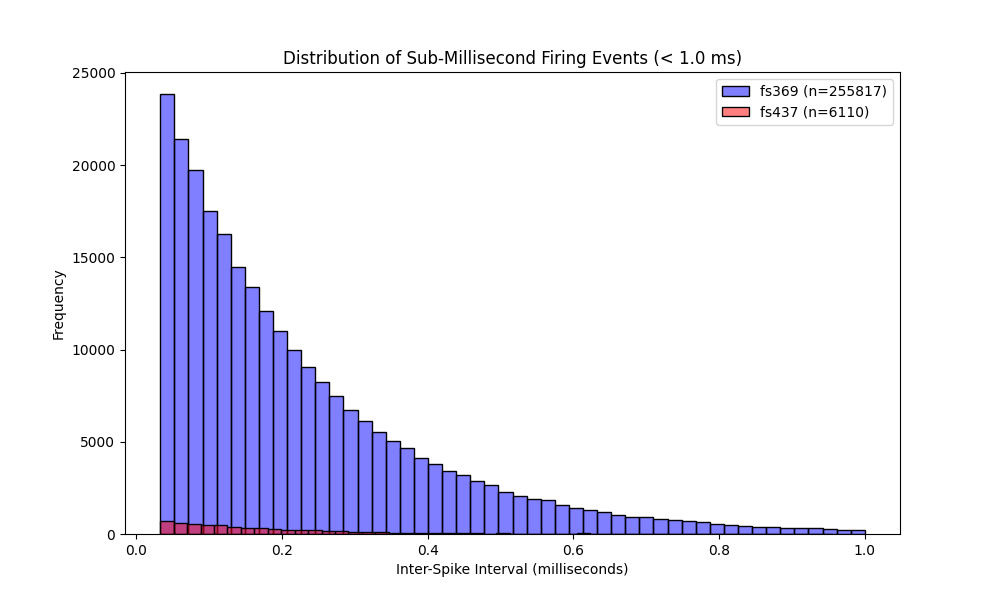
\includegraphics[width=0.8\textwidth]{sub_ms_burst_distribution.png}
\caption{Distribution of Sub-Millisecond Firing Events shifted by the 0.033 ms physical hardware limit.}
\label{fig:bursts}
\end{figure}

\section{Discussion}
The absolute minimum temporal bound of 0.033 ms mathematically confirms the physical Epistemological Detection Floor of standard 30 kHz MEAs. Because current sensors are inherently incapable of resolving phenomena below the microsecond scale, hypothesized quantum-scale biological phenomena operating at the femtosecond ($10^{-15}$ s) or picosecond ($10^{-12}$ s) scales cannot be empirically observed or verified within standard OI architectures. 

Consequently, the isolated ultra-fast network bursts must be driven by highly rapid classical mechanisms. The most biologically plausible explanations include direct electrical coupling via gap junctions or spatial multi-unit signal overlap, as standard neurotransmitter diffusion operates on a slower 1-2 ms scale. Furthermore, the profound K-S variance (K-S Statistic: 0.347, $p < 10^{-300}$) underscores extreme Developmental Divergence between the organoids, demonstrating massive structural or functional plasticity across the differing lifecycles.

\section{Methodological Limitations}
We acknowledge critical limitations within this methodological framework. The lack of spatial MEA mapping prevents the definitive dissociation between isolated single-unit hyper-firing and the overlapping detection of multiple adjacent soma. Future validation of the electrical synapse hypothesis strongly requires the integration of gap junction blockers (such as carbenoxolone). Additionally, while the 6xMAD dynamic thresholding provides robust artifact rejection, future analyses must meticulously parameterize the corresponding noise margins to ensure extreme frequency bursts are perfectly resolved from background electrical resonance.

\section{Conclusion}
This study characterizes the presence of ultra-fast sub-millisecond network dynamics in macro-scale neural organoids, mapping a definitive detection limit for electrophysiological recording platforms. We attribute the observed $< 1.0$ ms bursting divergence to structural developmental plasticity and classical biological mechanisms such as electrical coupling. Ultimately, establishing the 33.3-microsecond epistemological detection floor is vital for the integrity of Organoid Intelligence research; directly probing sub-classical biocomputing mechanisms will strictly require future deployment of high-bandwidth, gigahertz-scale sensory architectures.

\end{document}
